\documentclass{article}
\usepackage{amsmath} % For math environments if needed
\usepackage{geometry} % For adjusting margins
\geometry{a4paper, margin=1in}
\usepackage{enumitem} % For better lists
\usepackage{pgfplots} % For plotting graphs with TikZ and PGFPlots
\pgfplotsset{compat=1.17}
\usepackage{tikz}
\usepackage{gensymb}

\title{Economics 101: Problem Set \#7 Solutions}
\author{Sean Balbale}
\date{\today}

\begin{document}
\maketitle

% =============================================================
\section*{Problem 1: The 2001 Recession Case Study}
This problem is based on the final historical case study from the handout on ``Four Case Studies with the Aggregate Expenditures Model.'' It examines the U.S. recession of 2001.

\subsection*{Part (i): Explanation}
\begin{itemize}
  \item \textbf{Decline in Planned Gross Investment Expenditures:}\\
  During the 2001 recession, business expectations about future profitability declined sharply. This was largely a result of the bursting of the dot-com bubble, deteriorating market conditions, and increased uncertainty in the financial markets. With lower expected returns, firms reduced their planned gross investment expenditures.
  
  \item \textbf{Drop in Planned Consumption Expenditures:}\\
  At the same time, households experienced a fall in wealth due to collapsing asset values, and uncertainty about future income increased. This led consumers to postpone or scale back spending, so planned consumption expenditures also dropped.
\end{itemize}

\subsection*{Part (ii): AE--Y Diagram and Explanation}
The decline in both planned investment (\(I\)) and planned consumption (\(C\)) caused the Aggregate Expenditures (AE) curve to shift downward, from \(AE_0\) to \(AE_1\). This shift reflects the decrease in autonomous spending. The initial equilibrium was at or near potential GDP, denoted \(Y_P\). However, the downward shift in AE led to a new, lower equilibrium level of real GDP, denoted \(Y_{E1}\) (with equilibrium point \(E_1\)). The recessionary gap—the shortfall between full-employment output and the actual level of output—is given by 
\[
Y_P - Y_{E1} = 5,
\]
which reflects the \$5 billion gap identified in the text. In other words, during the 2001 recession the economy was producing less than its full-employment capacity.

\begin{center}
 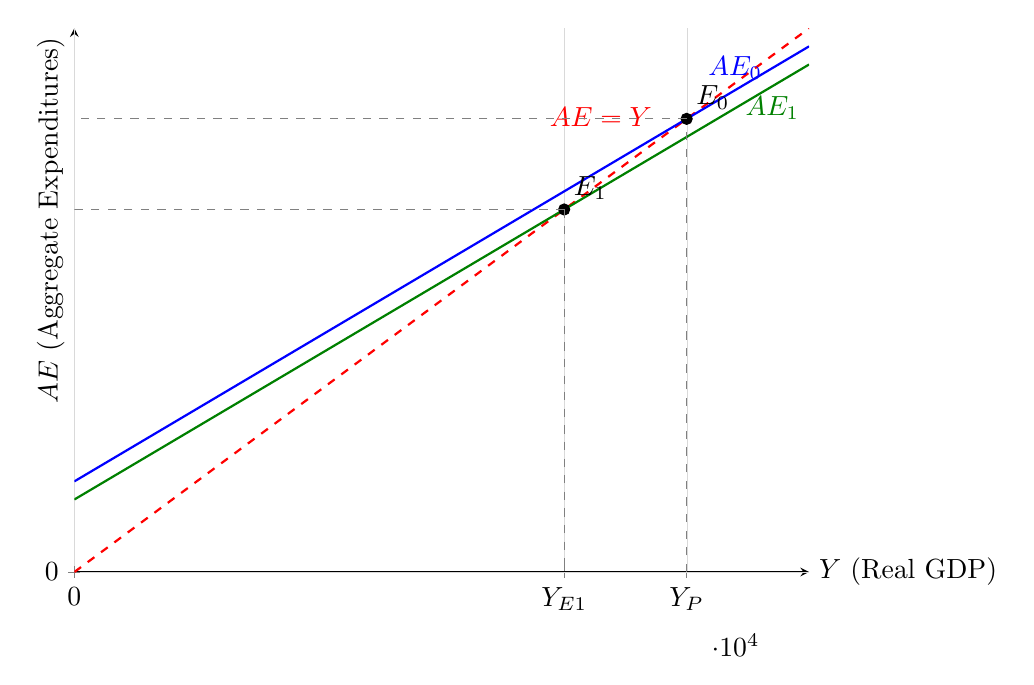
\begin{tikzpicture}
    \begin{axis}[
        width=0.9\textwidth, % Slightly wider
        height=0.7\textwidth, % Slightly taller
        xlabel={$Y$ (Real GDP)},
        ylabel={$AE$ (Aggregate Expenditures)},
        xmin=0, xmax=12000, % Adjusted limits for clarity
        ymin=0, ymax=12000, % Adjusted limits for clarity
        xtick={8000, 10000}, % Symbolic positions for Y_E1, Y_P
        xticklabels={$Y_{E1}$, $Y_P$},
        ytick=\empty, % No y-axis ticks needed for symbolic representation
        extra x ticks={0}, extra x tick labels={$0$},
        extra y ticks={0}, extra y tick labels={$0$},
        legend pos=north west,
        grid=major, % Major grid lines only
        grid style={line width=.1pt, draw=gray!30},
        axis lines=left, % Only bottom and left axis lines
        xlabel style={at=(current axis.right of origin), anchor=west},
        ylabel style={at=(current axis.above origin), anchor=south east},
        ]
      % 45-degree line (AE = Y)
      \addplot[
        domain=0:12000,
        samples=2, % Only need 2 points for a straight line
        red,
        dashed,
        thick % Make lines thicker
      ] {x} node[pos=0.8, anchor=south east, rotate=0] {$AE = Y$};

      % Initial AE curve (AE0) - Higher intercept, equilibrium at Y_P
      \addplot[
        domain=0:12000,
        samples=2, % Only need 2 points for a straight line
        blue,
        thick % Make lines thicker
        % Assume slope 0.8, Yp=10000. Y = AE = A + 0.8Y -> 0.2Y = A. At Y=10000, A=2000. AE0 = 2000 + 0.8Y
      ] {2000 + 0.8*x} node[anchor=east, pos=0.95] {$AE_0$};

      % New AE curve (AE1) - Lower intercept due to decreased C & I, equilibrium at Y_E1
      \addplot[
        domain=0:12000,
        samples=2, % Only need 2 points for a straight line
        green!50!black, % Different color
        thick % Make lines thicker
        % Assume Y_E1=8000. Y = AE = A' + 0.8Y -> 0.2Y = A'. At Y=8000, A'=1600. AE1 = 1600 + 0.8Y
      ] {1600 + 0.8*x} node[anchor=north, pos=0.95] {$AE_1$};

       % Potential GDP line (Y_P) - Vertical dashed line
      \draw[dashed, gray] (axis cs:10000, 0) -- (axis cs:10000, 10000);

      % Equilibrium points E0 and E1
      \filldraw[black] (axis cs:10000, 10000) circle (2pt) node[anchor=south west] {$E_0$}; % Equilibrium for AE0 at Y_P
      \filldraw[black] (axis cs:8000, 8000) circle (2pt) node[anchor=south west] {$E_1$}; % Equilibrium for AE1 at Y_E1

      % Dashed lines to axes for equilibrium points
      \draw[dashed, gray] (axis cs:10000, 10000) -- (axis cs:0, 10000); % E0 to y-axis (optional)
      \draw[dashed, gray] (axis cs:8000, 8000) -- (axis cs:8000, 0); % E1 to x-axis
      \draw[dashed, gray] (axis cs:8000, 8000) -- (axis cs:0, 8000); % E1 to y-axis (optional)

      % Annotate vertical shift (Decrease in autonomous expenditures)
      % \draw [-latex, thick] (axis cs:4000, 1600 + 0.8*4000 + 100) -- (axis cs:4000, 2000 + 0.8*4000 -100) node [midway, right, text width=2cm] {Decrease in autonomous C and I};

       % Annotate Recessionary Gap (using brace)
       \draw [decorate, decoration={brace, amplitude=10pt, mirror}, yshift=-5pt]
        (axis cs:8000,0) -- (axis cs:10000,0) node [black, midway, yshift=-15pt]
        {Recessionary Gap};

    \end{axis}
 \end{tikzpicture}
\end{center}
\textit{Note: Slopes and intercepts are illustrative. The key elements are the downward shift from \(AE_0\) to \(AE_1\) and the resulting equilibrium \(Y_{E1}\) being less than potential GDP \(Y_{P}\).}




% =============================================================
\section*{Problem 2: Stimulus Package to Boost Equilibrium Output}
In 2010, Congress was worried that the recovery might peter out and leave the economy below full employment. A stimulus package was proposed to increase government spending in order to boost aggregate expenditures and raise equilibrium output by \$500 billion.

\subsection*{Given:}
\[
\begin{aligned}
a &= 300\text{ billion} \quad\text{(autonomous consumption)} \\
b &= 0.90\quad\text{(marginal propensity to consume)} \\
T &= 50\text{ billion (lump sum taxes)} \\
I &= 350\text{ billion}, \quad G=250\text{ billion}, \quad X=40\text{ billion}, \quad M=45\text{ billion.}
\end{aligned}
\]

\subsection*{Step-by-Step Solution:}
\begin{enumerate}[label=\arabic*.]
  \item \textbf{Determine Autonomous Expenditures (AE intercept):}\\[1mm]
    The consumption function is given by: 
    \[
      C = a + b(Y-T) = 300 + 0.90(Y-50).
    \]
    For the AE function (which includes investment, government spending, and net exports):
    \[
    \begin{aligned}
      AE &= C + I + G + (X - M) \\
         &= \left[300 - 0.90\cdot50\right] + I + G + (X-M) + 0.90Y \\
         &= \left[300 - 45\right] + 350 + 250 + (40-45) + 0.90Y \\
         &= 255 + 350 + 250 - 5 + 0.90Y \\
         &= 850 + 0.90Y.
    \end{aligned}
    \]
  \item \textbf{Find Initial Equilibrium Output (\(Y_0\)):}\\[1mm]
    Equilibrium is where \(AE = Y\):
    \[
      Y = 850 + 0.90Y \quad \Rightarrow \quad 0.10Y = 850 \quad \Rightarrow \quad Y_0 = \frac{850}{0.10} = 8500\text{ billion}.
    \]
  \item \textbf{Determine the Required Increase in \(G\):}\\[1mm]
    The government spending multiplier (with no crowding out) is:
    \[
      k = \frac{1}{1-b} = \frac{1}{1-0.90} = 10.
    \]
    To increase \(Y\) by \$500 billion,
    \[
      \Delta G = \frac{\Delta Y}{k} = \frac{500}{10} = 50\text{ billion}.
    \]
  \item \textbf{New AE Function:}\\[1mm]
    With the increase in government spending, new \(G = 250 + 50 = 300\) billion, so the new autonomous part becomes:
    \[
    \begin{aligned}
      AE' &= [300 - 45] + 350 + 300 + (40-45) + 0.90Y \\
          &= 255 + 350 + 300 - 5 + 0.90Y \\
          &= 900 + 0.90Y.
    \end{aligned}
    \]
  \item \textbf{New Equilibrium Output (\(Y_1\)):}\\[1mm]
    Set \(Y = AE'\):
    \[
      Y = 900 + 0.90Y \quad \Rightarrow \quad 0.10Y = 900 \quad \Rightarrow \quad Y_1 = \frac{900}{0.10} = 9000\text{ billion}.
    \end{equation*}
\end{enumerate}

\subsection*{Explanation:}
Increasing government spending by \$50 billion shifts the AE function upward (from \(850+0.90Y\) to \(900+0.90Y\)). With a multiplier of 10, this raises equilibrium output by \$500 billion (from 8500 to 9000 billion dollars).

\subsection*{AE--Y Diagram}
\begin{center}
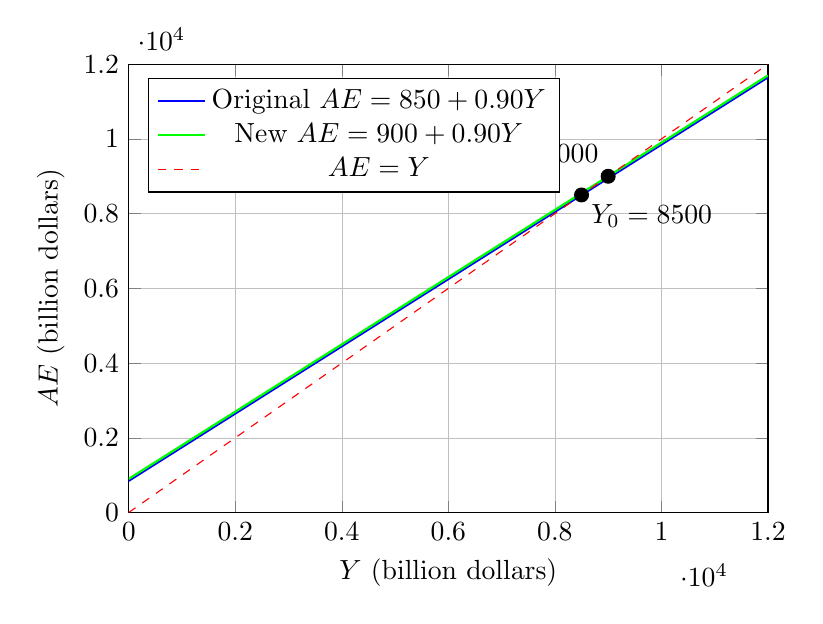
\begin{tikzpicture}
  \begin{axis}[
      width=0.8\textwidth,
      height=0.6\textwidth,
      xlabel={\(Y\) (billion dollars)},
      ylabel={\(AE\) (billion dollars)},
      xmin=0, xmax=12000,
      ymin=0, ymax=12000,
      xtick={0,2000,4000,6000,8000,10000,12000},
      ytick={0,2000,4000,6000,8000,10000,12000},
      legend pos=north west,
      grid=both,
      grid style={line width=.1pt, draw=gray!30},
      major grid style={line width=.2pt,draw=gray!50},
  ]
    % Original AE curve: AE = 850 + 0.90Y
    \addplot[
      domain=0:12000,
      samples=100,
      thick,
      blue
    ] {850 + 0.9*x};
    \addlegendentry{Original \(AE = 850+0.90Y\)}
    
    % New AE curve: AE = 900 + 0.90Y
    \addplot[
      domain=0:12000,
      samples=100,
      thick,
      green
    ] {900 + 0.9*x};
    \addlegendentry{New \(AE = 900+0.90Y\)}
    
    % 45-degree line: AE = Y
    \addplot[
      domain=0:12000,
      samples=100,
      dashed,
      red
    ] {x};
    \addlegendentry{\(AE = Y\)}
    
    % Mark original equilibrium: solve Y = 850 + 0.9Y -> Y=8500.
    \addplot[
      only marks,
      mark=*,
      mark size=2.5,
      black
    ] coordinates {(8500,8500)};
    \node[below right] at (axis cs:8500,8500) {\(Y_0=8500\)};
    
    % Mark new equilibrium: Y = 900 + 0.9Y -> Y=9000.
    \addplot[
      only marks,
      mark=*,
      mark size=2.5,
      black
    ] coordinates {(9000,9000)};
    \node[above left] at (axis cs:9000,9000) {\(Y_1=9000\)};
  \end{axis}
\end{tikzpicture}
\end{center}

% =============================================================
\section*{Problem 3: Tax Increase to Cool an Overheating Economy}
In 2018, Congress was concerned that the economy was overheating—that is, actual GDP was approaching or exceeding the full-employment level. To cool the economy, a policy of increasing personal (lump sum) taxes was considered. The goal was to reduce equilibrium output by \$180 billion.

\subsection*{Given:}
\[
\begin{aligned}
a &= 300\text{ billion} \quad\text{(autonomous consumption)} \\
b &= 0.80 \quad\text{(marginal propensity to consume)} \\
T &= 50\text{ billion} \quad\text{(lump sum taxes)} \\
I &= 350\text{ billion}, \quad G=250\text{ billion}, \quad X=40\text{ billion}, \quad M=45\text{ billion.}
\end{aligned}
\]

\subsection*{(A) Current Equilibrium GDP Calculation:}
\begin{enumerate}[label=\arabic*.]
  \item \textbf{Determine the Autonomous Component:}\\[1mm]
    Consumption is given by:
    \[
      C = a + b(Y-T) = 300 + 0.80(Y-50).
    \]
    The autonomous part from consumption is:
    \[
      a - bT = 300 - 0.80 \times 50 = 300 - 40 = 260.
    \]
    Adding the other autonomous expenditures:
    \[
      I + G + (X-M) = 350 + 250 + (40-45) = 350 + 250 - 5 = 595.
    \]
    So, total autonomous expenditure:
    \[
      A = 260 + 595 = 855.
    \]
  \item \textbf{Find Equilibrium Output:}\\[1mm]
    The AE function is:
    \[
      AE = A + bY = 855 + 0.80Y.
    \]
    Equilibrium (where \(Y = AE\)) is:
    \[
      Y = 855 + 0.80Y \quad \Rightarrow \quad 0.20Y = 855 \quad \Rightarrow \quad Y = \frac{855}{0.20} = 4275\text{ billion}.
    \]
\end{enumerate}
Thus, the current equilibrium GDP is 4275 billion dollars.

\subsection*{(B) Determining the Required Tax Increase:}
An increase in lump sum taxes, \(\Delta T\), affects consumption via the term \(-b\Delta T\). The new autonomous component becomes:
\[
  A' = \left[300 - b(T+\Delta T)\right] + (I+G+(X-M)) = \left[300 - bT\right] - b\Delta T + 595.
\]
Since initially \(300 - bT = 260\), we have:
\[
  A' = 260 - b\Delta T + 595 = 855 - b\Delta T.
\]
The new equilibrium output is:
\[
  Y' = \frac{A'}{1-b} = \frac{855 - b\Delta T}{1-b}.
\]
We want the equilibrium to decrease by 180 billion, i.e.,
\[
  Y - Y' = \frac{855}{1-b} - \frac{855 - b\Delta T}{1-b} = \frac{b\Delta T}{1-b} = 180.
\]
Solving for \(\Delta T\):
\[
  \Delta T = \frac{180(1-b)}{b}.
\]
Substitute \(b=0.80\):
\[
  \Delta T = \frac{180(1-0.80)}{0.80} = \frac{180(0.20)}{0.80} = \frac{36}{0.80} = 45\text{ billion}.
\]
So, taxes should be increased by \$45 billion.

\subsection*{Explanation:}
Increasing lump sum taxes reduces disposable income and hence consumption by \(b\Delta T\). The tax multiplier in this framework is \(-\frac{b}{1-b}\), so an increase of \$45 billion in taxes results in a decrease in equilibrium output by:
\[
  \Delta Y = -\frac{0.80}{0.20} \times 45 = -4 \times 45 = -180\text{ billion}.
\]
Thus, the desired reduction of \$180 billion in equilibrium output is achieved.

\subsection*{AE--Y Diagram}
\begin{center}
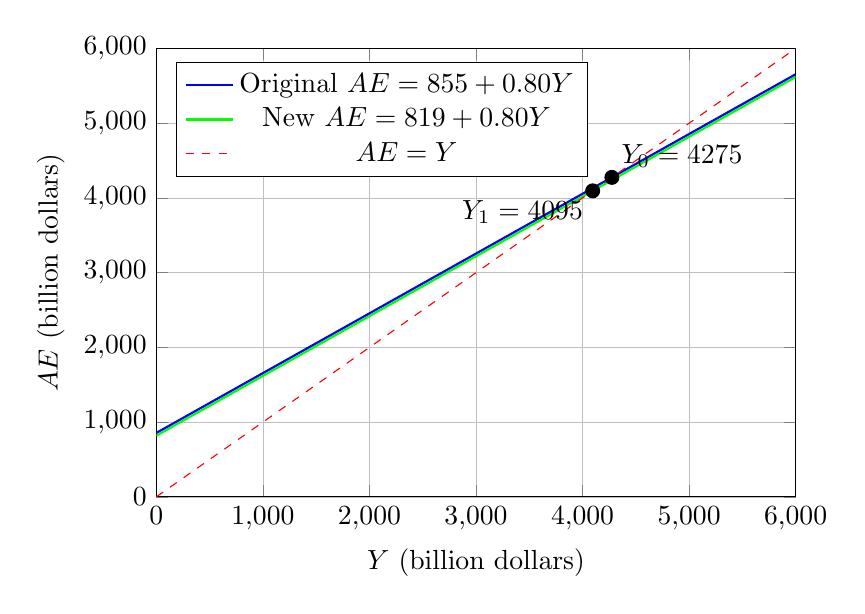
\begin{tikzpicture}
  \begin{axis}[
      width=0.8\textwidth,
      height=0.6\textwidth,
      xlabel={\(Y\) (billion dollars)},
      ylabel={\(AE\) (billion dollars)},
      xmin=0, xmax=6000,
      ymin=0, ymax=6000,
      xtick={0,1000,2000,3000,4000,5000,6000},
      ytick={0,1000,2000,3000,4000,5000,6000},
      legend pos=north west,
      grid=both,
      grid style={line width=.1pt, draw=gray!30},
      major grid style={line width=.2pt,draw=gray!50},
  ]
    % Original AE: AE = 855 + 0.80Y
    \addplot[
      domain=0:6000,
      samples=100,
      thick,
      blue
    ] {855 + 0.8*x};
    \addlegendentry{Original \(AE = 855+0.80Y\)}
    
    % New AE after tax increase (ΔT = 45): AE' = (855 - 0.80*45) + 0.80Y = (855 - 36) + 0.80Y = 819 + 0.80Y
    \addplot[
      domain=0:6000,
      samples=100,
      thick,
      green
    ] {819 + 0.8*x};
    \addlegendentry{New \(AE = 819+0.80Y\)}
    
    % 45-degree line: AE = Y
    \addplot[
      domain=0:6000,
      samples=100,
      dashed,
      red
    ] {x};
    \addlegendentry{\(AE = Y\)}
    
    % Mark original equilibrium: Y = 855/(0.20) = 4275
    \addplot[
      only marks,
      mark=*,
      mark size=2.5,
      black
    ] coordinates {(4275,4275)};
    \node[above right] at (axis cs:4275,4275) {\(Y_0=4275\)};
    
    % Mark new equilibrium: Y = 819/(0.20) = 4095
    \addplot[
      only marks,
      mark=*,
      mark size=2.5,
      black
    ] coordinates {(4095,4095)};
    \node[below left] at (axis cs:4095,4095) {\(Y_1=4095\)};
  \end{axis}
\end{tikzpicture}
\end{center}

\textbf{Overall Explanation:} The increase in lump sum taxes by \$45 billion reduces disposable income and thereby consumption spending. Through the multiplier effect (with multiplier \(=\frac{1}{1-b}\)), the equilibrium GDP falls from 4275 billion to 4095 billion dollars—a reduction of 180 billion dollars—thus cooling the economy to help dampen inflationary pressures.

\end{document}
